\documentclass[]{article}
\usepackage{aheader}
%\usepackage{theapa}
\usepackage{epsfig}
%\usepackage{amsmath}
\usepackage{amssymb}
\usepackage{fancyhdr}
\usepackage{algorithm}
\usepackage[noend]{algorithmic}
%\usepackage[algoruled,linesnumbered]{algorithm2e}

%%%%% Page Formatting: 

\pagestyle{fancy}
\lhead{}
\chead{Title}
\rhead{}
\lfoot{KSU Reasoning Group}
\cfoot{\thepage}
\rfoot{\today}
\renewcommand{\headrulewidth}{0.4pt}
\renewcommand{\footrulewidth}{0.4pt}

%%%%% Misc : 

\newcommand\shrink[1]{}
\def \definedas {{\:\:\:\:\stackrel{{\it{def}}}{=}\:\:\:\:}}
\def \questioneq {{\:\stackrel{{?}}{=}\:}}
\def\eproof{{\hfill$\Box$}}
\newenvironment{proof}[1][Proof]
			   {\begin{trivlist}\item[\hskip \labelsep {\bfseries #1}]}
			   {~\eproof \end{trivlist}}

\def\eql(#1,#2){{#1\!\!=\!#2}}

%%%%% ED stuff : 

\def\edkl{{\sc ed-kl}}
\def\edbp{{\sc ed-bp}}

\def\clone(#1){\hat{#1}}
\def\edse(#1){{{\it SE}(#1)}}
\def\edpm(#1){{{\it PM}(\clone(#1))}}
%\def\pse(#1,#2,#3){{{\it SE}^{#2}_{#3}(#1)}}
%\def\ppm(#1,#2,#3){{{\it PM}^{#2}_{#3}(#1)}}

%%%%% BN stuff

\def\gm{{\mathcal{M}}}
\def\gmp{{\mathcal{M}^\prime}}
\def\gme{{\mathcal{E}}}
\def\gmep{{\mathcal{E}^\prime}}

\def\bn{{\mathcal{N}}}
\def\bnp{{\mathcal{N}^\prime}}

\def\n(#1){\bar{#1}}
\def\p{{\bf p}}
\def\P{{\bf P}}
\def\s{{\bf s}}
\def\S{{\bf S}}

\def\u{{\bf u}}
\def\U{{\bf U}}
\def\v{{\bf v}}
\def\V{{\bf V}}
\def\x{{\bf x}}
\def\X{{\bf X}}
\def\y{{\bf y}}
\def\Y{{\bf Y}}
\def\z{{\bf z}}
\def\Z{{\bf Z}}
\def\e{{\bf e}}
\def\E{{\bf E}}
\def\ep{{\bf e^\prime}}
\def\Ep{{\bf E^\prime}}

\def\pr{{\it Pr}}
\def\prp{{\it Pr^\prime}}
\def\prh{\widehat{\it Pr}}

\def\bel{{\it BEL}}
\def\mi{{\it MI}}
\def\ent{{\it ENT}}
\def\kl{{\it KL}}
\def\ind{{\it IND}}

\newcommand\name[1]{\ensuremath{\mathsf{#1}}}
\def\true{\name{true}}
\def\false{\name{false}}

%%%%% complexity

\def\NP{{\mathrm{NP}}}
\def\PP{{\mathrm{PP}}}
\def\NPPP{{\NP^{\PP}}}

\newtheorem{theorem}{Theorem}
\newtheorem{corollary}{Corollary}
\newtheorem{lemma}{Lemma}
\newtheorem{definition}{Definition}
\newtheorem{proposition}{Proposition}
\newtheorem{claim}{Claim}
\newtheorem{condition}{Condition}
\newtheorem{conjecture}{Conjecture}

\author{Author}


\usepackage{amsmath}
\usepackage{graphicx}
\usepackage{color}

\newcommand{\art}[1]{{\color{red} \textit{[Art: #1~]}}}
\newcommand{\aadarsh}[1]{{\color{blue} \textit{[Aadarsh: #1~]}}}

%\def\equiv{{\bf EQUIV}}
\def\data{\mathcal{D}}
%hello
\chead{Testing Equivalence}

\begin{document}

%https://support.gurobi.com/hc/en-us/articles/4414392016529-How-do-I-model-conditional-statements-in-Gurobi

\subsection*{Verify that a Threshold Test is Always Passing}

\textbf{Definition.} Consider a threshold test of the following form:
\[
w_1 X_1 + w_2 X_2 + w_3 X_3 \ge T
\]
where \(X_1\), \(X_2,\) and \(X_3\) are binary variables, and \(w_1,\) \(w_2,\) \(w_3,\) and \(T\) are integer constants.

If this threshold test passes for any possible setting of the binary variables, then we say it is \emph{always passing}.

\textbf{Example.} Consider two different threshold tests:
\[
2 X_1 + X_2 - X_3 \ge -1
\mbox{ \quad\quad\quad\quad }
2 X_1 + X_2 - X_3 \ge 0.
\]
The left one is always passing.  The right one is not always passing, since it fails when \(X_1=0\), \(X_2=0\) and \(X_3=1\).

\textbf{Solution.}  We want to verify whether this test is always passing or not.  Consider the following optimization problem:
\begin{center}
\begin{tabular}{rl}
minimize   & \(Z\) \\
subject to & 
  $Z = 1$ \mbox{\quad if \quad} $w_1 X_1 + w_2 X_2 + w_3 X_3 \ge T$ \\
& $Z = 0$ \mbox{\quad if \quad} $w_1 X_1 + w_2 X_2 + w_3 X_3 \le T-1$ \\
& $X_1,X_2,X_3,Z$ are binary
\end{tabular}
\end{center}
Note that the first two constraints are indicator constraints.  Note further that if \(a\) and \(b\) are integers, then \(a < b\) if and only if \(a \le b-1\).\footnote{Note that Gurobi does not support strict inequality constraints.  However, a strict inequality constraint over integers can be emulated by a non-strict one.}  Hence, the first indicator constraint asserts that \(Z=1\) if the threshold test passes, and the second indicator constraint asserts that \(Z=0\) if the threshold test fails.

The objective is to minimize $Z$.  That is, we ask if $Z$ is ever equal to 0?  If so, then the threshold test can fail.  If $Z$ can never be 0, then it is always 1, and thus the threshold test always passes.

\newpage
\subsection*{Verify the Equivalence of Two Threshold Tests}

\textbf{Definition.} Consider two threshold tests of the following form:
\[
w_1 X_1 + w_2 X_2 + w_3 X_3 \ge T
\]
\[
w'_1 X_1 + w'_2 X_2 + w'_3 X_3 \ge T'
\]
where \(X_1\), \(X_2\), and \(X_3\) are binary variables, and \(w_1\), \(w_2\), \(w_3\), \(T\), \(w'_1\), \(w'_2\), \(w'_3\), and \(T'\) are integer constants.

We are interested in determining whether these two threshold tests are equivalent, meaning they always yield the same result for any possible setting of the binary variables.

\textbf{Example 1 (Not Equivalent).} Consider the following two threshold tests:
\[
2 X_1 + X_2 - X_3 \ge 1
\mbox{ \quad\quad\quad\quad }
X_1 + 2X_2 - X_3 \ge 0.
\]
To verify if these two tests are not equivalent, we can construct a truth table for all possible combinations of \(X_1\), \(X_2\), and \(X_3\):

\[
\begin{array}{|c|c|c|c|c|}
\hline
X_1 & X_2 & X_3 & \text{Test 1} & \text{Test 2} \\
\hline
0 & 0 & 0 & 0 & 0 \\ \hline
0 & 0 & 1 & 0 & 0 \\ \hline
0 & 1 & 0 & 0 & 1 \\ \hline
0 & 1 & 1 & 0 & 0 \\ \hline
1 & 0 & 0 & 1 & 1 \\ \hline
1 & 0 & 1 & 0 & 0 \\ \hline
1 & 1 & 0 & 1 & 1 \\ \hline
1 & 1 & 1 & 1 & 1 \\ 
\hline 
\end{array}
\]

From the truth table, we see that there is at least one configuration (\(X_1 = 0\), \(X_2 = 1\), \(X_3 = 0\)) where Test 1 and Test 2 yield different results. Therefore, these two threshold tests are not equivalent.

\textbf{Example 2 (Equivalent).} Consider the following two threshold tests:
\[
2 X_1 + 2 X_2 - 2 X_3 \ge 0
\mbox{ \quad\quad\quad\quad }
2 X_1 + 2 X_2 - 2 X_3 \ge -1.
\]
To verify if these two tests are equivalent, we can construct a truth table for all possible combinations of \(X_1\), \(X_2\), and \(X_3\):

\[
\begin{array}{|c|c|c|c|c|}
\hline
X_1 & X_2 & X_3 & \text{Test 1} & \text{Test 2} \\
\hline
0 & 0 & 0 & 1 & 1 \\ \hline
0 & 0 & 1 & 0 & 0 \\ \hline
0 & 1 & 0 & 1 & 1 \\ \hline
0 & 1 & 1 & 1 & 1 \\ \hline
1 & 0 & 0 & 1 & 1 \\ \hline
1 & 0 & 1 & 1 & 1 \\ \hline
1 & 1 & 0 & 1 & 1 \\ \hline
1 & 1 & 1 & 1 & 1 \\ 
\hline
\end{array}
\]

From the truth table, we see that Test 1 and Test 2 yield the same result for all possible combinations of \(X_1\), \(X_2\), and \(X_3\). Therefore, these two threshold tests are equivalent.

In essence, this test showcases from \(Z_1\) and \(Z_2\) being binary, it has the following behavior:
\[
(Z_1 \wedge \neg Z_2) \vee (\neg Z_1 \wedge Z_2)
\]
where \(\wedge\) is conjunction (logical-AND), \(\vee\) is disjunction (logical-OR), and \(\neg X\) means negation of \(X\) or not \(X\). Hence, through Gurobi's algebraic logic, it satisfies this condition by stating if \(Z_1 + Z_2 == 1\), then the thresholds are inequivalent.

% ARTHUR: we can test equivalence by performing two implication tests, i.e, we can test whether "if T1 passes then T2 passes" and whether "if T2 passes then T1 passes" and if both are true, then they are equivalent.

\newpage
\subsection*{Verify the Equivalence of Two Threshold-Tests (Quadratic Program)}

\textbf{Definition.} 

\art{The below looks like part of the solution, not the definition of the problem we are trying to solve. (Which is equivalence in this case)}

This code evaluates the equivalence of two threshold-based tests using Gurobi's optimization framework. The primary focus is on constructing two linear expressions:
\[
test1\_expr = w_1 X_1 + w_2 X_2 + w_3 X_3
\]
\[
test2\_expr = w'_1 X_1 + w'_2 X_2 + w'_3 X_3
\]
that represent the outcomes of each test based on the binary variables \(X_1\), \(X_2\), and \(X_3\), and their associated weights \(w_1\), \(w_2\), \(w_3\), \(w'_1\), \(w'_2\), and \(w'_3\). The threshold values \(T\) and \(T'\) determine when each test passes.

\textbf{Example.} Consider the following weights and thresholds:
\[
w_1 = 2, \quad w_2 = 1, \quad w_3 = -1, \quad T = 1
\]
\[
w'_1 = 1, \quad w'_2 = 2, \quad w'_3 = -1, \quad T' = 0
\]
Then the expressions become:
\[
test1\_expr = 2 X_1 + X_2 - X_3
\]
\[
test2\_expr = X_1 + 2 X_2 - X_3
\]

Instead of directly comparing the results, the code introduces two modified expressions, \(f_1\) and \(f_2\):
\[
f_1 = test1\_expr - T + k_1
\]
\[
f_2 = test2\_expr - T' + k_2
\]
where \(k_1\) and \(k_2\) are constants that adjust the test outcomes. 

\art{\(k = \frac{1}{2}\) and explain why we need that.}
The constants \(k_1\) and \(k_2\) are introduced to normalize or offset the expressions to ensure they can be effectively compared. For instance, setting \(k_1 = \frac{1}{2}\) helps to establish a baseline for comparison, ensuring that the linear combinations of the binary variables can be adequately evaluated relative to their respective thresholds. Namely, when the test expression and the threshold are the same, equating to 0, the k value ensures its positive value, making sure of it's equivalence or in-equivalence. This is particularly important when the weights and thresholds are not aligned, as it allows for a more nuanced assessment of equivalence.

These modified expressions are then multiplied, with the product serving as the objective to be minimized:
\[
\text{Objective: } f_1 \cdot f_2
\]

The goal is to find an input configuration where this product leads to the conclusion that the tests are either equivalent or not. 

\textbf{Solution.} If the model finds an optimal solution such that the product is minimized, it indicates that the tests are equivalent; otherwise, they are not. When \(f_1\) and \(f_1\) are both positive, it assesses its equivalence, if not vice versa.



\newpage
Suppose we have two threshold tests:
\begin{equation} \label{eq:1}
w_1 x_1 + w_2 x_2 + w_3 x_3 \ge T
\end{equation}
and
\begin{equation} \label{eq:2}
w'_1 x_1 + w'_2 x_2 + w'_3 x_3 \ge T'
\end{equation}
Test~\ref{eq:1} has one set of weights \(w_1,w_2\) and \(w_3\) and threshold \(T\).  Test~\ref{eq:2} has another set of weights \(w'_1,w'_2\) and \(w'_3\) and threshold \(T'\).  Both tests have the same set of binary inputs \(x_1,x_2\) and \(x_3\), i.e., they can be either 0 or 1.

Let \(f_1\) be the function representing Test~\ref{eq:1} and let \(f_2\) be the function representing Test~\ref{eq:2}.  We say that Test~\ref{eq:1} is \emph{equivalent} to Test~\ref{eq:2} if and only if 
\[
f_1(x_1,x_2,x_3) = f_2(x_1,x_2,x_3)
\]
for all possible settings of the inputs \(x_1,x_2\) and \(x_3\).  In other words, the truth table of Test~\ref{eq:1} has the same rows as the truth table of Test~\ref{eq:2}.

For example, the threshold test
\begin{equation} \label{eq:3}
4 \cdot x_1 + 2 \cdot x_2 - 4 \cdot x_3 \ge 1
\end{equation}
is equivalent to the threshold test
\begin{equation} \label{eq:4}
4 \cdot x_1 + 2 \cdot x_2 - 4 \cdot x_3 \ge 2
\end{equation}
but both are in equivalent to the threshold test
\begin{equation} \label{eq:5}
4 \cdot x_1 + 2 \cdot x_2 - 4 \cdot x_3 \ge 3
\end{equation}
as they differ on input setting \((x_1,x_2,x_3) = (0,1,0).\)  Tests~\ref{eq:3} and \ref{eq:4} pass on this input whereas Test~\ref{eq:5} fails.

Next, we say that Test 1 \emph{covers} Test 2 if and only if
\[
f_1(x_1,x_2,x_3) \ge f_2(x_1,x_2,x_3)
\]
for all possible settings of the inputs \(x_1,x_2\) and \(x_3\).  In other words, if Test 2 passes then Test 1 also passes.  That is, if \(f_2(x_1,x_2,x_3) = 1\) then \(f_1(x_1,x_2,x_3) = 1\).  Equivalently, if Test 1 fails, then Test 2 also fails (the contrapositive).

If Test 1 covers Test 2 and Test 2 covers Test 1, then Test 1 and Test 2 are equivalent.

TODO: can you write up and explain the quadratic program example?  include some examples

\newpage

\subsection*{Threshold Test Example}

\textbf{Definition.} Consider a threshold test of the following form:
\[
w_1 X_1 + w_2 X_2 + w_3 X_3 \ge T
\]
where \(X_1\), \(X_2,\) and \(X_3\) are binary variables, and \(w_1,\) \(w_2,\) \(w_3,\) and \(T\) are integer constants.

%Additionally, let a second threshold test be defined similarly as:
%\[
%w'_1 X_1 + w'_2 X_2 + w'_3 X_3 \ge T_p
%\]
%where \(T_p\) is a variable threshold to be maximized.

\begin{figure}
    \centering
    \includegraphics[width=\textwidth]{Screenshot 2024-11-01 at 1.26.08 PM.png}
    \caption{Caption}
    \label{fig:enter-label}
\end{figure}

Located in this figure, we are observing the lower bound (the highest inequivalent expression prior to change in behavior). Given this threshold test, what is the largest value of \(T\) that does not change the behavior of the threshold test.  Or equivalently, what is the largest value of \(T\) that results in an equivalent threshold test.

\textbf{Example.} Consider the following thresholds and weights:
\[
\begin{aligned}
    & w_1 = 2, w_2 = 2, w_3 = -2, \\
%    & w'_1 = 2, w'_2 = 2, w'_3 = -2, \\
    & T = 1
\end{aligned}
\]
Consider the following truth table:

%\textbf{Truth Table for \(T = 1\):}
\[
\begin{array}{|c|c|c|c|c|c|c|}
\hline
X_1 & X_2 & X_3 & 2X_1 + 2X_2 - 2X_3 & \ge 1? & \ge 2? & \ge 3? \\
\hline
0 & 0 & 0 & 0 & 0 & 0 & 0 \\ \hline
0 & 0 & 1 & -2 & 0 & 0 & 0 \\ \hline
0 & 1 & 0 & 2 & 1 & 1 & 0 \\ \hline
0 & 1 & 1 & 0 & 0 & 0 & 0 \\ \hline
1 & 0 & 0 & 2 & 1 & 1 & 0 \\ \hline
1 & 0 & 1 & 0 & 0 & 0 & 0 \\ \hline
1 & 1 & 0 & 4 & 1 & 1 & 1 \\ \hline
1 & 1 & 1 & 2 & 1 & 1 & 0 \\
\hline
\end{array}
\]
Here, the test passes (i.e., returns 1) when the threshold is met or exceeded.

Next, we maximize the threshold \(T\) to determine the largest value that maintains the same behavior.


Initially, by increasing the threshold test by 1, we see that the behavior remains the same when \(T = 2\). 

However, when the threshold is 3, in this case, the behavior has changed. Specifically, for the rows where \(X_1 = 0, X_2 = 1, X_3 = 0\) and \(X_1 = 1, X_2 = 0, X_3 = 0\), the threshold test now fails. Therefore, the largest value of \(T\) that maintains the behavior is \(T = 2\).

\textbf{Solution.} We model this as an optimization problem using binary variables \(X_1, X_2, X_3, Z_1, Z_2\), where:
\begin{center}
\begin{tabular}{rl}
minimize   & \(T_p\) \\
subject to & 
  $Z_1 = 1$ \mbox{\quad if \quad} $2 X_1 + 2 X_2 - 2 X_3 \ge T$ \\
& $Z_1 = 0$ \mbox{\quad if \quad} $2 X_1 + 2 X_2 - 2 X_3 \le T-1$ \\
& $Z_2 = 1$ \mbox{\quad if \quad} $2 X_1 + 2 X_2 - 2 X_3 \ge T_p$ \\
& $Z_2 = 0$ \mbox{\quad if \quad} $2 X_1 + 2 X_2 - 2 X_3 \le T_p-1$ \\
& $Z_1 + Z_2 = 1$ \mbox{\quad (exactly one  of the thresholds must pass)} \\
& $T_p \ge T$ \\
& $X_1, X_2, X_3, Z_1, Z_2 \in \{0,1\}$, and $T_p \in \mathbb{Z}$
\end{tabular}
\end{center}

\art{argue that if \(T_p\)  = 1 then the constraints are infeasible (in particular Z1 + Z2 = 1 is infeasible.  \(T_p\) =2 it is still feasible,  = 0) \(T_p\)=3 it and \(X_1 = 1, X_2 = 0, X_3 = 0\), this feasible.  The idea is for all \(T_p\) >= T, some settings of \(T_p\) are feasible (threshold test now fails. Therefore, the largest value of \(T\) that maintains the behavior is \(T = 2\).}

The problem becomes infeasible when \( T_p = 1 \) because both \( Z_1 = 1 \) and \( Z_2 = 1 \) would need to hold simultaneously, which violates the constraint \( Z_1 + Z_2 = 1 \). In particular, for \( Z_1 = 1 \), the constraint \( 2X_1 + 2X_2 - 2X_3 \geq 1 \) is infeasible with \( X_1 = 1, X_2 = 0, X_3 = 0 \), and for \( Z_2 = 1 \), the constraint \( 2X_1 + 2X_2 - 2X_3 \geq T_p = 1 \) is also satisfied. However, this would force both \( Z_1 \) and \( Z_2 \) to be 1, which contradicts \( Z_1 + Z_2 = 1 \). When \( T_p = 2 \), the constraints remains infeasible since the settings \( X_1 = 1, X_2 = 0, X_3 = 0 \) satisfy both \( Z_1 = 1 \) (where \( 2X_1 + 2X_2 - 2X_3 \geq 1 \)) and \( Z_2 = 0 \) (where \( 2X_1 + 2X_2 - 2X_3 \leq T_p - 1 = 1 \)). Therefore, the model is feasible. For \( T_p = 3 \), the configuration \( X_1 = 1, X_2 = 0, X_3 = 0 \) satisfies \( Z_1 = 1 \), but does not satisfy \( Z_2 = 1 \) since \( 2X_1 + 2X_2 - 2X_3 = 2 \) is not greater than or equal to \( T_p = 3 \). Thus, the largest value of \( T_p \) that maintains the feasibility of the constraints is \( T_p = 2 \), and for all \( T_p \geq T \), some settings of \( X_1, X_2, X_3 \) are infeasible.


\textbf{Conclusion/Solution.} The largest threshold \(T_p\) that maintains the same behavior of the original threshold test is \(T_p = 2\). When \(T_p = 3\), the behavior changes as demonstrated in the truth table tests are in-equivalent) and others are infeasible (the tests are equivalent).  So when you minimize \(T_p\), you we are looking for the transition when the tests go from in-equivalent to equivalent.

Note that the first two constraints are indicator constraints: the first one asserts that \(Z_1 = 1\) if the first threshold test passes, and the second asserts that \(Z_2 = 1\) if the second threshold test passes. The third constraint enforces that only one threshold test passes at a time. 

In addition, there is another constraint stating that \(T_p\) is greater than T.

The goal is to minimize \(T_p\) under these constraints. If \(T_p\) reaches its minimum value and the threshold tests are still passing, then the test is valid for this threshold (maintaining the same behavior).


\newpage
\subsection*{Threshold Minimization Problem with Gurobi}

\textbf{Definition.} We define a threshold test of the following form:
\[
w_1 X_1 + w_2 X_2 + w_3 X_3 \ge T
\]
where \(X_1\), \(X_2\), and \(X_3\) are binary variables, and \(w_1\), \(w_2\), \(w_3\), and \(T\) are integer constants. Additionally, we define a second threshold test as follows:
\[
w'_1 X_1 + w'_2 X_2 + w'_3 X_3 \ge T_p
\]
where \( T_p \) is a variable threshold representing an upper bound, which we aim to maximize while maintaining the same feasible behavior as in the original threshold test.

The objective is to minimize \( T_p \), to the upper bound of its equivalence, ensuring that the threshold test's behavior remains consistent.

\textbf{Example.} Consider the following weights and threshold:
\[
\begin{aligned}
    & w_1 = 10, \quad w_2 = 15, \quad w_3 = -5, \\
    & w'_1 = 10, \quad w'_2 = 15, \quad w'_3 = -5, \\
    & T = 20
\end{aligned}
\]
Now, let us examine the behavior of the test by constructing a truth table for various values of \( T \) and \( T_p \):

\[
\begin{array}{|c|c|c|c|c|c|c|}
\hline
X_1 & X_2 & X_3 & 10X_1 + 15X_2 - 5X_3 & \ge 20? & \ge 25? & \ge 30? \\
\hline
0 & 0 & 0 & 0 & 0 & 0 & 0 \\ \hline
0 & 0 & 1 & -5 & 0 & 0 & 0 \\ \hline
0 & 1 & 0 & 15 & 0 & 0 & 0 \\ \hline
0 & 1 & 1 & 10 & 0 & 0 & 0 \\ \hline
1 & 0 & 0 & 10 & 0 & 0 & 0 \\ \hline
1 & 0 & 1 & 5 & 0 & 0 & 0 \\ \hline
1 & 1 & 0 & 25 & 1 & 1 & 0 \\ \hline
1 & 1 & 1 & 20 & 1 & 0 & 0 \\ 
\hline
\end{array}
\]
Here, the test passes (returns 1) for certain configurations of \(X_1\), \(X_2\), and \(X_3\) when \( T = 20 \) or \( T = 25 \), but fails at \( T = 30 \).

\textbf{Solution.} We model this as an optimization problem with Gurobi using binary variables \(X_1, X_2, X_3, Z_1, Z_2\), where we aim to maximize \( T_p \) subject to the following constraints:

\begin{center}
\begin{tabular}{rl}
\text{minimize}   & \( T_p \) \\ 
\text{subject to} & 
  \( Z_1 = 1 \) \quad if \quad \( 10 X_1 + 15 X_2 - 5 X_3 \ge T \), \\
                  & \( Z_1 = 0 \) \quad if \quad \( 10 X_1 + 15 X_2 - 5 X_3 \le T - 1 \), \\
                  & \( Z_2 = 1 \) \quad if \quad \( 10 X_1 + 15 X_2 - 5 X_3 \ge T_p \), \\
                  & \( Z_2 = 0 \) \quad if \quad \( 10 X_1 + 15 X_2 - 5 X_3 \le T_p - 1 \), \\
                  & \( Z_1 + Z_2 = 1 \) \quad (only one threshold test can be active at a time), \\
                  & \( T_p \ge T \), \\
                  & \( X_1, X_2, X_3, Z_1, Z_2 \in \{0,1\} \), \( T_p \in \mathbb{Z} \).
\end{tabular}
\end{center}

The first two constraints define indicator conditions: \( Z_1 = 1 \) if the original threshold \( T \) is met or exceeded, and \( Z_2 = 1 \) if the variable threshold \( T_p \) is met or exceeded. The constraint \( Z_1 + Z_2 = 1 \) ensures only one of the threshold conditions holds.

\textbf{Conclusion.} By solving this minimization problem, we identify the smallest feasible \( T_p \) that behaves consistently with the initial threshold test defined by \( T \). This setup allows us to determine the minimal threshold that maintains equivalent feasible configurations across both tests.

\begin{figure}
    \centering
    \includegraphics[width=\textwidth]{Screenshot 2024-11-01 at 1.26.08 PM.png}
    \label{fig:enter-label}
\end{figure}

\end{document}






\newpage
to do: minimize the thresold, attempting to find the minimal, maintaining the same behavior.

Consider the following threshold test:
\begin{equation} \label{eq:example}
4 \cdot I_1 + 2 \cdot I_2 - 4 \cdot I_3 \ge 1.
\end{equation}
Here, \(I_1, I_2\) and \(I_3\) are our inputs, and each can be either 0 or 1.  The threshold test either passes or it fails.  We can use a function \(f\) to describe the behavior of this threshold test, where \(f(I_1,I_2,I_3) = 1\) if the test passes, and \(f(I_1,I_2,I_3) = 0\) if it fails.

We can enumerate all possible inputs and record the output, as we would a truth table:
\begin{center}
\small
\begin{tabular}{ccc|r|c}
$I_1$ & $I_2$ & $I_3$ & sum & $f$ \\\hline
    0 &     0 &     0 &  0 & 0 \\
    0 &     0 &     1 & -4 & 0 \\
    0 &     1 &     0 &  2 & 1 \\
    0 &     1 &     1 & -2 & 0
\end{tabular}
\quad\quad
\begin{tabular}{ccc|r|c}
$I_1$ & $I_2$ & $I_3$ & sum & $f$ \\\hline
    1 &     0 &     0 &  4 & 1 \\
    1 &     0 &     1 &  0 & 0 \\
    1 &     1 &     0 &  6 & 1 \\
    1 &     1 &     1 &  2 & 1
\end{tabular}.
\end{center}
Here, the ``sum'' column is the sum that results on the left-hand-side of the threshold test.

In general, say we we have a threshold test over 3 inputs:
\begin{equation} \label{eq:threshold}
w_1 \cdot I_1 + w_2 \cdot I_2 + w_3 \cdot I_3 \ge T.
\end{equation}
where \(w_1\), \(w_2\) and \(w_3\) are the weights of the thersold test, and \(T\) is the thresold.  Assume that all of these parameters are integers.


\textbf{Questions:} (about the initial threshold test)
\begin{enumerate}
\item Identify another value of the thershold \(T\) that results in an equivalent threshold test (where the truth table has the same output values for \(f\)).
\item Identify another value of the weight \(w_1\) that results in an equivalent threshold test.
\item What is the range of values \([a,b]\) for the threshold \(T\) that results in an equivalent threshold test?
\item What is the range of values \([a,b]\) for the threshold \(w_1\) that results in an equivalent threshold test?
\end{enumerate}

%{
%\bibliographystyle{plain}
%\bibliography{refs}
%}


Here is a figure:
\begin{center}
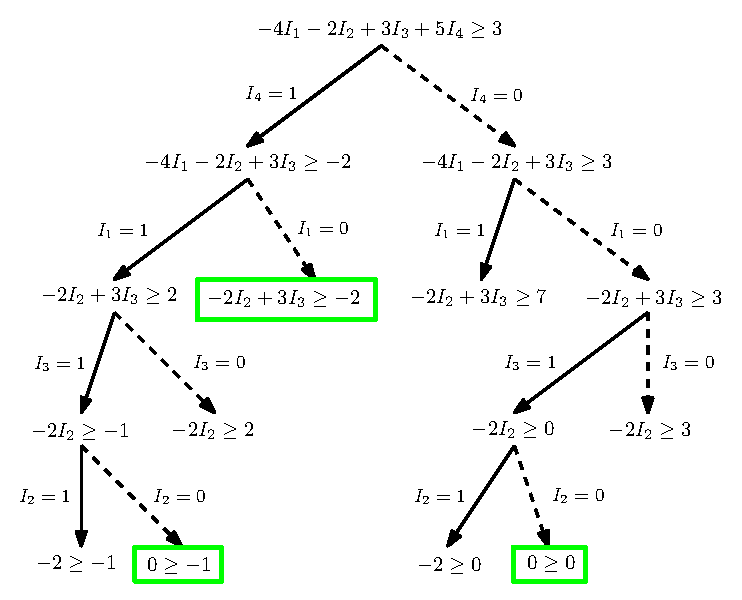
\includegraphics[width=.9\linewidth]{figs/digitsdecisiontree}
\end{center}


\end{document}
